\documentclass{article}
\usepackage[paperwidth=7.16in,paperheight=8.0in,margin=0pt]{geometry}
\usepackage{graphicx}
\usepackage{tikz}
\usetikzlibrary{calc,matrix}
\pagestyle{empty}
\setlength{\parindent}{0pt}

% Discrete stops sampled from Matplotlib's cyclic twilight map.  The raster
% phase panels use the full Matplotlib map; these stops draw the TikZ bars.
\definecolor{phasea}{RGB}{68,1,84}
\definecolor{phaseb}{RGB}{60,78,137}
\definecolor{phasec}{RGB}{35,140,141}
\definecolor{phased}{RGB}{65,182,130}
\definecolor{phasee}{RGB}{148,213,96}
\definecolor{phasef}{RGB}{221,202,76}
\definecolor{phaseg}{RGB}{238,128,55}
\definecolor{phaseh}{RGB}{184,55,121}

\newcommand{\panel}[1]{\includegraphics[width=1.48in,height=1.48in]{#1}}
\newcommand{\ticklabel}[2]{\node[anchor=north,font=\scriptsize] at (#1, -0.02in) {#2};}
\newcommand{\graybar}[4]{%
  \begin{tikzpicture}[baseline=(current bounding box.north)]
    \shade[left color=black,right color=white] (0,0) rectangle (1.48in,0.09in);
    \draw[gray!55,line width=0.2pt] (0,0) rectangle (1.48in,0.09in);
    \node[anchor=north west,font=\scriptsize] at (0in,-0.02in) {0};
    \node[anchor=north,font=\scriptsize] at (0.74in,-0.02in) {#2};
    \node[anchor=north east,font=\scriptsize] at (1.48in,-0.02in) {#3};
    \node[anchor=north,align=center,text width=1.48in,font=\scriptsize] at (0.74in,-0.24in) {#4};
  \end{tikzpicture}%
}
\newcommand{\phasebar}{%
  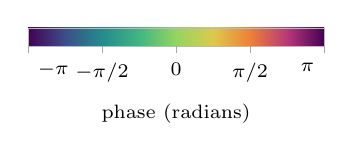
\begin{tikzpicture}[baseline=(current bounding box.north)]
    \shade[left color=phasea,right color=phaseb] (0in,0) rectangle (0.185in,0.09in);
    \shade[left color=phaseb,right color=phasec] (0.185in,0) rectangle (0.370in,0.09in);
    \shade[left color=phasec,right color=phased] (0.370in,0) rectangle (0.555in,0.09in);
    \shade[left color=phased,right color=phasee] (0.555in,0) rectangle (0.740in,0.09in);
    \shade[left color=phasee,right color=phasef] (0.740in,0) rectangle (0.925in,0.09in);
    \shade[left color=phasef,right color=phaseg] (0.925in,0) rectangle (1.110in,0.09in);
    \shade[left color=phaseg,right color=phaseh] (1.110in,0) rectangle (1.295in,0.09in);
    \shade[left color=phaseh,right color=phasea] (1.295in,0) rectangle (1.480in,0.09in);
    \draw[gray!55,line width=0.2pt] (0,0) rectangle (1.48in,0.09in);
    \draw[gray!70,line width=0.25pt] (0in,0) -- ++(0,-0.035in);
    \draw[gray!70,line width=0.25pt] (0.37in,0) -- ++(0,-0.035in);
    \draw[gray!70,line width=0.25pt] (0.74in,0) -- ++(0,-0.035in);
    \draw[gray!70,line width=0.25pt] (1.11in,0) -- ++(0,-0.035in);
    \draw[gray!70,line width=0.25pt] (1.48in,0) -- ++(0,-0.035in);
    \node[anchor=north west,font=\scriptsize] at (0in,-0.035in) {$-\pi$};
    \node[anchor=north,font=\scriptsize] at (0.37in,-0.035in) {$-\pi/2$};
    \node[anchor=north,font=\scriptsize] at (0.74in,-0.035in) {$0$};
    \node[anchor=north,font=\scriptsize] at (1.11in,-0.035in) {$\pi/2$};
    \node[anchor=north east,font=\scriptsize] at (1.48in,-0.035in) {$\pi$};
    \node[anchor=north,font=\scriptsize] at (0.74in,-0.24in) {phase (radians)};
  \end{tikzpicture}%
}

\begin{document}
\centering
\begin{tikzpicture}
  \matrix (grid) [
    matrix of nodes,
    nodes in empty cells,
    row sep=0.025in,
    column sep=0.045in,
    inner sep=0pt,
    nodes={inner sep=0pt, outer sep=0pt}
  ] {
    \panel{image_magnitude_coil1.png} & \panel{image_phase_coil1.png} & \panel{fourier_log_magnitude_coil1.png} & \panel{fourier_phase_coil1.png} \\
    \panel{image_magnitude_coil2.png} & \panel{image_phase_coil2.png} & \panel{fourier_log_magnitude_coil2.png} & \panel{fourier_phase_coil2.png} \\
    \panel{image_magnitude_coil3.png} & \panel{image_phase_coil3.png} & \panel{fourier_log_magnitude_coil3.png} & \panel{fourier_phase_coil3.png} \\
    \panel{image_magnitude_coil4.png} & \panel{image_phase_coil4.png} & \panel{fourier_log_magnitude_coil4.png} & \panel{fourier_phase_coil4.png} \\
  };

  \node[above=2pt, align=center, font=\scriptsize\bfseries] at (grid-1-1.north) {\textbf{(a)}\\[-1pt]Image-domain magnitude};
  \node[above=2pt, align=center, font=\scriptsize\bfseries] at (grid-1-2.north) {\textbf{(b)}\\[-1pt]Image-domain phase};
  \node[above=2pt, align=center, font=\scriptsize\bfseries] at (grid-1-3.north) {\textbf{(c)}\\[-1pt]Fourier-domain log magnitude};
  \node[above=2pt, align=center, font=\scriptsize\bfseries] at (grid-1-4.north) {\textbf{(d)}\\[-1pt]Fourier-domain phase\\[-1pt](centered 50\% crop)};

  \foreach \row/\label in {1/Coil 1,2/Coil 2,3/Coil 3,4/Coil 4} {
    \node[anchor=east, font=\scriptsize] at ([xshift=-0.09in]grid-\row-1.west) {\label};
  }

  \node[anchor=north] at ([yshift=-0.14in]grid-4-1.south) {\graybar{1.0791}{0.5396}{1.0791}{scaled magnitude}};
  \node[anchor=north] at ([yshift=-0.14in]grid-4-2.south) {\phasebar};
  \node[anchor=north] at ([yshift=-0.14in]grid-4-3.south) {\graybar{0.9443}{0.4722}{0.9443}{log magnitude (display scale)}};
  \node[anchor=north] at ([yshift=-0.14in]grid-4-4.south) {\phasebar};
\end{tikzpicture}

\vspace{0.25in}
\begin{minipage}{7.0in}
\scriptsize
\textbf{Figure 1.} Representative prepared T2-weighted slice showing the four selected receiver coils after phase alignment and shared robust scaling. Phase hue denotes angle on a cyclic $[-\pi,\pi]$ scale. Image-domain phase is shown at near-full opacity within the foreground support, whereas Fourier phase uses magnitude-weighted opacity and a centered 50\% crop of k-space; the Fourier log magnitude remains full-frame. These visualization choices do not change the model input, which uses the centered orthonormal FFT and shared robust scaling from the experimental pipeline.
\end{minipage}
\end{document}
